\chapter{Desenvolvimento}
%-------------------------------------------------------------------
Este capítulo descreve as etapas realizadas para atingir os objetivos desse trabalho. O trabalho foi dividido em quatro etapas, dada a complexidade do \emph{framework} em questão, essa decisão foi tomada visando primeiramente entender o contexto ao qual o escalonador terá de se adaptar e de que forma isso será feito, deixando a etapa de implementação para o final quando todos os pré-requisitos para a inserção no \emph{Hadoop} já estiverem concluídos. A primeira etapa visou à instalação e configuração das versões 1.0.4 e 2.0.3 (YARN), para aprofundar o conhecimento sobre os requisitos do ambiente para que o \emph{framework} seja utilizado. Na segunda etapa foram feitas as instalações dos componentes necessários para a compilação do código, visto que o objetivo do trabalho é alterar o código fonte do Apache Hadoop. A terceira etapa foi destinada ao estudo da arquitetura do \emph{Apache Hadoop}, através do código dos escalonadores disponibilizados e da máquina de estados do \emph{Resource Manager}. Finalmente a quarta etapa é a de desenvolvimento do escalonador, o qual será posteriormente testado tanto em ambiente local como no Grid'5000.

%-------------------------------------------------------------------
\section{Configuração do ambiente de execução}
A instalação do \emph{Apache Hadoop}, ao contrário da instalação dos programas que usuários finais estão habituados, não possui interface gráfica. Na verdade a instalação não passa da extração dos arquivos para uma pasta, porém a configuração do ambiente não é trivial e exige um conhecimento de administração de sistemas e redes. 

Para o correto funcionamento do \emph{Apache Hadoop}, é necessária a edição de alguns arquivos que descrevem o ambiente no qual esse irá rodar. Além disso, é necessária a configuração de uma rede onde os nós possam se comunicar livremente. Sabendo que o \emph{Apache Hadoop} sofreu algumas alterações ao mudar da versão 1.x para o 2.x (YARN), esperava-se que ao realizar a instalação e configuração das duas versões, a identificação das diferenças entre elas torna-se mais simples.

No início do trabalho o objetivo era de instalar e configurar o \emph{Apache Hadoop} em três situações: 
\begin{itemize}
	\item \emph{localhost}, também chamado de \emph{single-node}
	\item \emph{mini cluster}, chamado de \emph{multi-node}
	\item Grid'5000, sendo também um caso de \emph{multi-node}
\end{itemize}

São duas as etapas de configuração, a configuração da rede e comunicação a qual é referente à configuração independente do hadoop, ou seja, são tarefas a serem realizadas dentro do sistema operacional, tal como a criação de usuário e configuração do ssh. Enquanto isso, a configuração do ambiente é referente à configuração específica do \emph{Apache Hadoop}, portanto têm de alterar arquivos de configuração dentro pasta de instalação desse de tal forma que ao serem executados, os deamons do \emph{Apache Hadoop} rodem sem problemas.

A configuração do sistema operacional é exatamente igual em ambas versões, desde a criação de um usuário exclusivo para o \emph{Apache Hadoop} até a criação das chaves públicas de SSH.

Quanto à configuração do ambiente existem algumas diferenças entre as versões, mas ambas seguem a mesma forma geral de configuração, com pequenas diferenças pontuais em alguns casos. Essa configuração é feita através da edição de arquivos xml, nos quais são inseridos propriedades com nome e valor, as quais irão alterar o funcionamento ou a classe específica que será utilizada na execução. A maior diferença entre as versões é a adição de um novo arquivo na versão YARN, que possui muitos parâmetros importantes, por se tratar da configuração do módulo do \emph{MapReduce}.

Inicialmente optou-se por configurar ambas as versões em todas as instâncias especificadas, porém devido ao foco do projeto a utilização da versão 1.x não seria mais interessante e foi descontinada.

A configuração no ambiente \emph{localhost}, é simples e ocorre sem problemas após um contato básico com o \emph{framework}. A partir desse ponto, a complexidade começa a aumentar, visto que são inseridos mais nós e existe a necessidade de um gerenciamento melhor, além da inserção de mais propriedades nos arquivos.

Para a versão \emph{mini cluster}, foram utilizadas duas máquinas, já apresentando uma diferença entre as versões. Na versão 1.x o mestre poderia também ser escravo, ou seja, uma máquina poderia ser \emph{NameNode, DataNode, TaskManager e TaskTracker}. Na versão YARN isso já muda e a máquina de gerenciamento não pode executar \emph{deamons} de processamento.

Para a configuração no Grid'5000, foi decidido utilizar somente a versão YARN. Uma vez que a versão \emph{mini cluster} já tinha sido configurada, foram necessárias poucas adaptações. A principal diferença foi quanto à configuração interna do Grid'5000, tendo que ser aplicadas ferramentas disponibilizadas para utilização e criação de imagens de sistema, além de algumas diferenças para obter os \emph{tarballs} necessários para os testes de instalação e execução, que só poderiam ser obtidos com wget através de um \emph{proxy} ou que se fosse alguma versão diferente da oficial, através de \emph{scp}.

Ao final desta etapa, alguns pontos do \emph{Hadoop} já tinham sido esclarecidos e também já havia sido estabelecido um ambiente de execução onde os testes serão feitos ao final da implementação. 

Ainda como resultado desta etapa, destaca-se a identificação de algumas peculiaridades do \emph{framework} que poderiam dificultar o trabalho, como o caso de inserção de um novo nó escravo. Para que esse nó seja inserido, os serviços tem de ser parados, para que o usuário altere o arquivo de escravos e então reinicie os serviços. O mesmo acontece para qualquer propriedade que deseja-se alterar nos arquivos \emph{xml}, não há possibilidade de alterá-las sem que os serviços sejam interrompidos e reiniciados.

%-------------------------------------------------------------------
\section{Alteração e compilação do código fonte}
Dada a natureza do projeto, de gerar um novo escalonador sensível ao contexto para o \emph{Apache Hadoop}, é necessário que esse escalonador seja incluído na distribuição final e que fique disponível para o uso de todos usuários que fizerem o \emph{download} da versão alterada.

Para que isso seja alcançado, é necessário gerar novos arquivos \emph{.jar} a partir do código fonte modificado, ou nesse caso, adicionado. Em razão disto foi feito um estudo prévio das etapas e requisitos necessários para a compilação e geração desses arquivos.

Primeiramente foi feita uma consulta à documentação oficial e aos arquivos de suporte inclusos nas distribuições do código fonte. Adquirindo-se assim um guia do que era necessário e quais as etapas a seguir.

Partindo da lista de requisitos nas fontes de informação, estes foram instalados. Alguns foram facilmente instalados pelo próprio gerenciador de pacotes do GNU outros requeriram um esforço maior, mas no geral esta etapa decorreu sem maiores problemas.

A última etapa era a compilação própriamente dita, onde bastava executar o comando do \emph{Apache Maven} \cite{Maven} e esperar enquanto ele fazia o download de requisitos e a construção dos arquivos executáveis. Existem alguns parâmetros que podem ser adicionados ou retirados no momento da compilação de acordo com a intenção do usuário, como por exemplo a opção de pular os testes, a opção de compilar código nativo e documentação, entre outras.

Houveram problemas na etapa de compilação própriamente dita, onde a ferramenta de compilação \emph{Apache Maven} causava alguns erros em função dos arquivos de configuração utilizados por ela (arquivos \emph{pom.xml}). Através de uma busca nos fóruns de desenvolvedor da comunidade \emph{Hadoop}, foi possível identificar que o erro era referente à versão de um dos requisitos (\emph{Protocol Buffer} \cite{protobuff}), o qual encontrava-se com uma versão desatualizada no arquivo de configuração, bastando alterar a versão ou aplicar o patch de correção disponibilizado pela equipe para que o erro fosse sanado.

Embora a compilação do código padrão tenha sido bem sucedida, o maior objetivo deste processo era descobrir como a compilação decorreria com a adição de novas classes no código padrão. Com vistas a atingir esse objetivo, uma nova classe de escalonador foi adicionada. Essencialmente essa classe era apenas uma cópia do escalonador FIFO renomeada e em outro \emph{package}. Após gerar os arquivos executáveis com a adição dessa nova classe, esses arquivos foram copiados para o Grid'5000 e foi feita uma nova instalação.

Com essa nova instalação em mãos, foi possível testar o funcionamento e compará-lo com o da distribuição padrão. Além disso foram feitos testes para que fosse comprovado a utilização do "novo" escalonador, os quais foram concluídos com sucesso, mediante uma linha extra de código identificando que o escalonador utilizado era essa versão alterada. Seguindo na mesma vulnerabilidade identificada na instalação do ambiente de execução, a opção de qual escalonador será utilizado é mediante arquivo \emph{xml} e também deve ser feita antes do serviço \emph{ResourceManager} ser iniciado, caso contrário esse serviço terá de ser parado e reiniciado.

%-------------------------------------------------------------------
\section{Estudo da arquitetura do \emph{Apache Hadoop}}
Com intuito de criar um escalonador sensível ao contexto é necessário que a arquitetura do \emph{Apache Hadoop} seja compreendida. Esta etapa do projeto tem objetivos de identificar as dependências entre as classes, além de quais classes serão necessárias implementar e como se dará essa implementação.

Uma vez que um escalonador funcional é uma implementação de uma série de classes abstratas e \emph{interfaces}, é um bom começo saber a origem de tais classes e o que cada uma irá influenciar na classe final. Ainda, através do estudo da arquitetura, é possível identificar os recursos disponibilizados pelo \emph{framework} para que então sejam decididas as estratégias de escalonamento.

Para o estudo da arquitetura foram utilizados dois métodos. O primeiro método empregado consistiu no estudo do próprio código enquanto o segundo pela geração e estudo de máquinas de estado do \emph{Resource Manager}. Esse passo foi destinado à identificação de todos os componentes de um escalonador, desde a identificação de quais \emph{interfaces} e classes abstratas foram implementadas até o estudo e investigação dos critérios de escalonamento e como estes são aplicados nos escalonadores disponibilizados.

Devido à complexidade do \emph{framework} decidiu-se por utilizar a \emph{IDE IntelliJIDEA} \cite{IDEA} na execução do primeiro método. Terminado o estudo do código, foi possível gerar um diagrama de classes daquelas que compõem um escalonador, o qual é apresentado na Figura \ref{fig:Diagrama de Classes}.

\begin{figure}[hbtn]
   \centering
   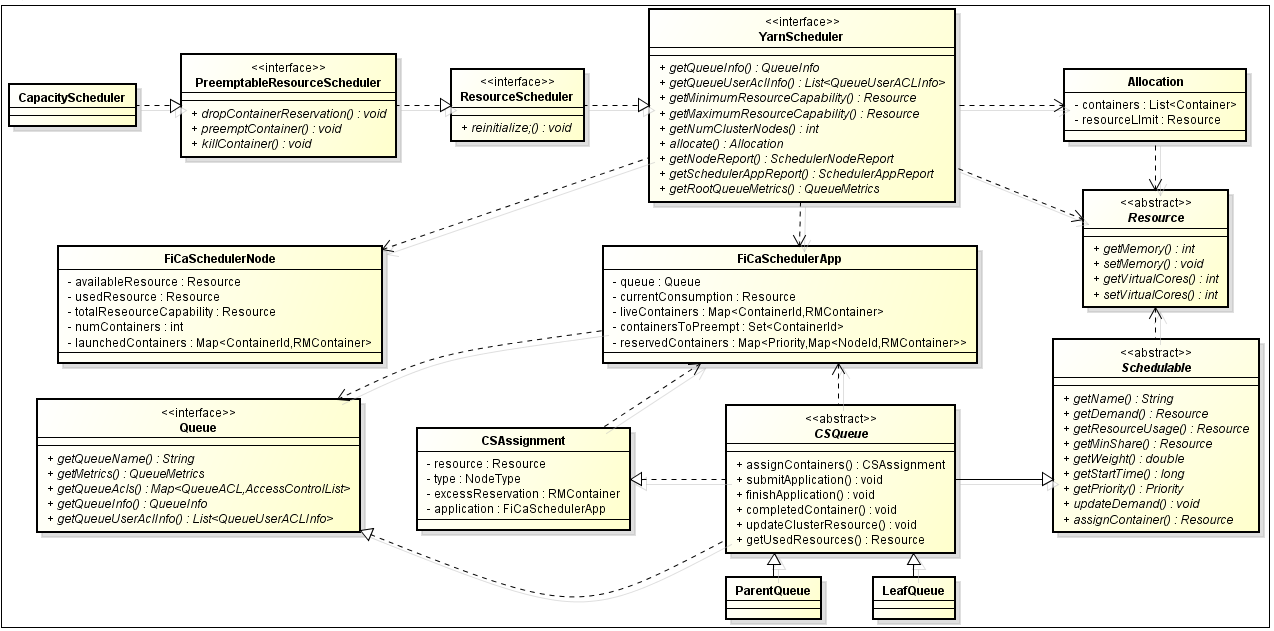
\includegraphics[width=15cm]{figuras/Figura01-ClassDiagram.png}
   \caption{Diagrama de classe com as principais classes que compõem o \emph{FairScheduler}}
   \label{fig:Diagrama de Classes}
\end{figure}

Identificou-se também a ideia base de cada componente, as quais serão explicadas a seguir:

\begin{itemize}
	\item \emph{Schedulable}: uma classe abstrata que representa uma entidade que pode lançar um \emph{job} ou uma \emph{queue}, disponibiliza uma interface simples pela qual os algoritmos podem ser aplicados tanto dentro de uma \emph{queue} quanto a várias delas.
	\item \emph{Queue}: uma \emph{interface} que possibilita o controle básico de todas as \emph{queues} de um escalonador.
	\item \emph{YarnScheduler}: outra \emph{interface} através da qual os componentes podem se comunicar com o escalonador, seja para alocar ou liberar recursos.
	\item \emph{Resource}: uma classe abstrata responsável por modelar os recursos de um computador (memória, cores etc.) a serem utilizados.
	\item \emph{Comparable}: uma \emph{interface} que possibilita comparar vários tipos de dados, utilizado para comparar os \emph{jobs} submetidos e ver qual tem prioridade segundo os critérios de escalonamento adotados.
\end{itemize}

O segundo método foi realizado mediante uma opção disponibilizada pelo próprio \emph{Maven}, em que é possível gerar grafos que representam as máquinas de estado referentes ao funcionamento do \emph{Resource Manager} e do \emph{Node Manager}. Este método apresentou como resultado os grafos referentes às máquinas de estados geradas a partir do \emph{Resource Manager}, é possível identificar que são máquinas de estado de sub-componentes dele. Ainda constata-se que as figuras podem ajudar a identificar o fluxo de um \emph{job}, o que será importante na etapa de testes em situações adversas. As figuras podem ser visualizadas no \autoref{chap:ApendA} do trabalho.

Terminada essa etapa, todos os requisitos necessários para a implementação já estão concluídos, já existe um ambiente de execução para os testes, já existe um ambiente de compilação e implementação do código, os recursos possíveis de serem utilizados já estão identificados e as alterações de configuração necessárias na instalação do \emph{Hadoop} para que um novo escalonador seja utilizado são conhecidas.